\documentclass[hidelinks, a4paper, 12pt]{article}
\usepackage[linktoc=all]{hyperref}
\usepackage{apacite}
\usepackage[margin=1.0in]{geometry}
\usepackage{amssymb}
\usepackage{amsmath}
\usepackage{amsthm}
\usepackage{pgfplots}
\pgfplotsset{compat=1.16}
\usepackage{tikz}
\usepackage{pgf}
\usepackage{mathrsfs}
\usepackage{array}
\usepackage{tabularx}
\usepackage{braket}

\allowdisplaybreaks


\hypersetup{
    pdftitle={The Weird and Wonderful World of the Qubit},
    pdfauthor={Wilson Wongso},
    pdfpagemode=UseOutlines,
}

\title{The Weird and Wonderful World of the Qubit}
\author{Notes taken by Wilson Wongso}
\date{}

\setcounter{section}{-1}
\setcounter{tocdepth}{2}

\graphicspath{ {./images/} }

\newcommand{\biimp}{\Leftrightarrow}
\newcommand{\bd}{\textbf}
\newcommand{\n}{\\[\baselineskip]}
\newcommand{\real}{\mathbb{R}}
\newcommand{\thus}{\Rightarrow}

\begin{document}

    \maketitle
        
    \tableofcontents

    \section{Preface}
        The following notes are based on the textbook \bd{Learn Quantum Computation Using Qiskit} \cite{Qiskit-Textbook}.
        The author simply wishes to compile a part of his learning journey into this document.

    \section{Qubit States}
        \subsection{The z basis}
            The z basis has two states, an initial state of \bd{0} and the other state of \bd{1}.
            If we do a z-measurement on any of these states, it is certain to output either a 0 or a 1.\n
            The two states can be denoted by two types of vectors, a column vector/ket-vector:
            \[\ket{0} = \begin{pmatrix} 1 \\ 0 \end{pmatrix}\]
            \[\ket{1} = \begin{pmatrix} 0 \\ 1 \end{pmatrix}\]
            or a row vector/bra-vector:
            \[\begin{split}
                \bra{0} &= \begin{pmatrix} 1 & 0 \end{pmatrix}\n
                \bra{1} &= \begin{pmatrix} 0 & 1 \end{pmatrix}
            \end{split}\]
            As vectors, these states can also undergo operations like any other ordinary vectors.

            \subsubsection{Addition of Vectors}
                \[\begin{pmatrix} a_0 \\ a_1 \end{pmatrix} + \begin{pmatrix} b_0 \\ b_1 \end{pmatrix} = \begin{pmatrix} a_0 + b_0 \\ a_1 + b_1 \end{pmatrix}\]

            \subsubsection{Multiplying by Scalar}
                \[c \times \begin{pmatrix} a_0 \\ a_1 \end{pmatrix} = \begin{pmatrix} c \times a_0 \\ c \times a_1 \end{pmatrix}\]

            \subsubsection{Multiplying with a Vector}
                \[\begin{pmatrix} a_0 & a_1 \end{pmatrix} \begin{pmatrix} b_0 \\ b_1 \end{pmatrix} = a_0 b_0 + a_1 b_1\]
            
            \subsubsection{Inner Product}
                An inner product requires one vector to be a bra-vector and the other to be a ket-vector.
                \[\begin{split}
                    \braket{0|0} = \braket{1|1} = 1\n
                    \braket{0|1} = \braket{1|0} = 0
                \end{split}\]
                \bd{Notice:} The inner product of the same state outputs a $1$ while the inner product of \bd{0} and \bd{1} is $0$, indicating that they are orthogonal to each other. 

        \subsection{The x basis - Part 1}
            We would like to find states for which the outcome of a z measurement is equally likely to be 0 or 1.\n
            A good place to start is from $\ket{0} + \ket{1}$ since this includes both $\ket{0}$ and $\ket{1}$ with no particular bias towards either.\n
            Multiply them with an $x$ and solve for the value of $x$ that would result in orthogonal and normalized states:
            \[x(\ket{0} + \ket{1}) = \begin{pmatrix} x \\ x \end{pmatrix}\]
            As we know, the inner product of the same state should result with a $1$ for it to be normalized, thus:
            \[\begin{split}
                \begin{pmatrix} x & x \end{pmatrix} \begin{pmatrix} x \\ x \end{pmatrix} &= 2x^2\n
                \thus 2x^2 &= 1\\
                x^2 &= \frac{1}{2}\\
                x &= \pm \frac{1}{\sqrt{2}}
            \end{split}\]
            Taking the value of $x = \frac{1}{\sqrt{2}}$, we can write down the new state as:
            \[\begin{pmatrix} \frac{1}{\sqrt{2}} \\ \frac{1}{\sqrt{2}} \end{pmatrix} = \frac{1}{\sqrt{2}} \begin{pmatrix} 1 \\ 1 \end{pmatrix} = \frac{\ket{0} + \ket{1}}{\sqrt{2}}\]
            This state is denoted by the ket vector $\ket{+}$, hence:
            \[\ket{+} = \frac{\ket{0} + \ket{1}}{\sqrt{2}}\]

        \subsection{The Born Rule}
            The inner product squared of $\ket{0}$, $\ket{1}$, and $\ket{+}$ respectively with $\bra{0}$ is equivalent with z measurement.
            \begin{center}
                \begin{tabular}{c c}
                $\braket{0|0} = 1$ & $\thus p_0^z(\ket{0}) = 1$\\
                \\
                $\braket{0|1} = 0$ & $\thus p_0^z(\ket{1}) = 1$\\
                \\
                $\braket{0|+} = \frac{1}{\sqrt{2}}$ & $\thus p_0^z(\ket{+}) = \frac{1}{2}$\\
               \end{tabular}
            \end{center}
            This property also applies with $\bra{1}$, thus the following relationships are true:
            \[\begin{split}
                p_0^z(\ket{a}) &= (\braket{0|a})^2\n
                p_1^z(\ket{a}) &= (\braket{1|a})^2\\
            \end{split}\]

        \subsection{Global and Relative Phases}
            Let $\ket{\tilde{0}}$ be the product of $\ket{0}$ with $-1$:
            \[\ket{\tilde{0}} = \begin{pmatrix}
                -1 \\ 0
            \end{pmatrix} = -\ket{0}\]
            This means, that every inner product we could calculate with $\ket{\tilde{0}}$ is the same as for $\ket{0}$, but multiplied by $-1$.
            \[\begin{split}
                \braket{a|\tilde{0}} &= -\braket{a|0}\n
                p^a = (\braket{a|\tilde{0}})^2 &= (\braket{a|0})^2
            \end{split}\]
            Therefore, there is no observable difference between $\ket{0}$ and $\ket{\tilde{0}}$, which is represents the irrelevance of global phase.\n
            While, if we only multiply one element in the vector, it creates a relative phase which creates an entirely different state.
            \[\begin{pmatrix} a_0 \\ a_1 \end{pmatrix} \rightarrow \begin{pmatrix} a_0 \\ -a_1 \end{pmatrix}\]
            Doing so with $\ket{+}$ state gives us a new state:
            \[\ket{-} = \frac{1}{\sqrt{2}} \begin{pmatrix} 1 \\ -1 \end{pmatrix} = \frac{\ket{0} - \ket{1}}{\sqrt{2}}\]
            The z measurement of $\ket{+}$ and $\ket{-}$ are the same, and they are orthogonal to each other:
            \[\braket{-|+} = \braket{+|-} = 0\]

        \subsection{The x basis - Part 2}
            Finding two orthogonal states allows us to define a new kind of measurement.\n
            In the z basis, anything but $\ket{0}$ and $\ket{1}$ is treated as a superposition of the two:
            \[\begin{split}
                \ket{+} &= \frac{\ket{0} + \ket{1}}{\sqrt{2}}\n
                \ket{-} &= \frac{\ket{0} - \ket{1}}{\sqrt{2}}
            \end{split}\]
            We can do the same with the x basis:
            \[\begin{split}
                \ket{0} &= \frac{\ket{+} + \ket{-}}{\sqrt{2}}\n
                \ket{1} &= \frac{\ket{+} - \ket{-}}{\sqrt{2}}
            \end{split}\]
            Hence the probability measurements:
            \[\begin{split}
                p_0^x (\ket{a}) &= (\braket{+|a})^2\n
                p_1^x (\ket{a}) &= (\braket{-|a})^2\n
            \end{split}\]

        \subsection{The y basis - Part 1}
            Similarly, we need another basis that is mutually unbiased with x and z to conserve certainty.
            \[\ket{\circlearrowleft} = c_0\ket{0} + c_1\ket{1}\]
            No real numbers would satisfy y basis, thus complex numbers are required.

        \subsection{Complex Numbers}
            A complex number is made up of a real and an imaginary part:
            \[x = x_r + ix_i\]
            It has a corresponding conjugate:
            \[x^* = x_r - ix_i\]
            And its magnitude:
            \[|x| = \sqrt{xx^*}\]
            Extending the bra-ket notation, its entries now allow for complex numbers. The ket vector is now defined as the following:
            \[\begin{split}
                \ket{a} &= \begin{pmatrix} a_0 \\ a_1 \end{pmatrix}\n
                \bra{a} &= \begin{pmatrix} a_0^* & a_1^* \end{pmatrix}
            \end{split}\]

        \subsection{Born Rule with Complex Numbers}
            Instead of squaring inner products, we need to square the magnitudes of the inner products:
            \[\begin{split}
                p_0^z(\ket{a}) &= |\braket{0|a}|^2\n
                p_1^z(\ket{a}) &= |\braket{1|a}|^2\n
                p_0^x(\ket{a}) &= |\braket{+|a}|^2\n
                p_1^x(\ket{a}) &= |\braket{-|a}|^2\n
            \end{split}\]

        \subsection{The y basis - Part 2}
            Now that we can utilize complex numbers, we find the two state vectors which are orthogonal to each other and mutually unbiased with x and z:
            \[\begin{split}
                \ket{\circlearrowright} &= \frac{\ket{0} + i\ket{1}}{\sqrt{2}}\n
                \ket{\circlearrowleft} &= \frac{\ket{0} - i\ket{1}}{\sqrt{2}}
            \end{split}\]

        \subsection{Heisenberg's Uncertainty Principle for Qubits}
            Whatever operations we apply, a single isolated qubit will always obey:
            \[(p_0^z - p_1^z)^2 + (p_0^x - p_1^x)^2 + (p_0^y - p_1^y)^2 = 1\]

    \section{Pauli Matrices and the Bloch Sphere}
        \subsection{Pauli Matrices}
            There are three important matrices for qubits are known as the Pauli matrices:
            \[\begin{split}
                X &= \begin{pmatrix} 0 & 1 \\ 1 & 0 \end{pmatrix}\n
                Y &= \begin{pmatrix} 0 & -i \\ i & 0 \end{pmatrix}\n
                Z &= \begin{pmatrix} 1 & 0 \\ 0 & -1 \end{pmatrix}
            \end{split}\]
            These have many useful properties, as well as a deep connection to the x, y and z measurements.\n
            Specifically, we can use them to calculate the three quantities used in the last section, namely the expectation values:
            \[\begin{split}
                \braket{a|X|a} &= p_0^x(\ket{a}) - p_1^x(\ket{a})\n
                \braket{a|Y|a} &= p_0^y(\ket{a}) - p_1^y(\ket{a})\n
                \braket{a|Z|a} &= p_0^z(\ket{a}) - p_1^z(\ket{a})\n
            \end{split}\]
            The compact notation of expectation values is normally used as the following:
            \[\braket{X} = \braket{a|X|a}\]
            Therefore, the compact notation for conservation of certainty is:
            \[\braket{X}^2 + \braket{Y}^2 + \braket{Z}^2 = 1\]

        \subsection{The Bloch Sphere}
            \bd{Notice:}
            \[-1 \leq \braket{X}, \braket{Y}, \braket{Z} \leq 1\]
            Knowing this property allows us to represent every point on the surface of a sphere in terms of its x, y and z coordinates.\n
            The coordinates are then constrained by the radius in both directions: they can be no greater than $r$ and no less than $-r$. We can set $r = 1$.\n
            Distance from the surface of the sphere can be determined by the 3D version of Pythagoras' theorem, $x^2 + y^2 + z^2$. 
            Points on the surface always have a distance of 1.\n
            \begin{figure}[ht]
                \centering
                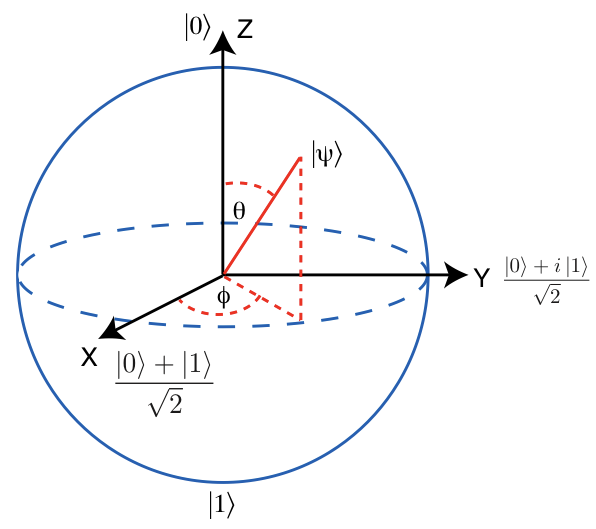
\includegraphics[scale=0.4]{bloch-sphere}
            \end{figure}\n
            We set $\ket{0}$ as north pole, $\ket{1}$ as south pole, and x, y measurements around the equator. Orthogonal states are also diametrically opposite.\n
            The Bloch Sphere makes it easier to understand single-qubit operations. Each moves points around on the surface of the sphere, and so can be interpreted as a simple rotation.

    \section{States for Many Qubits}
        \subsection{Two-qubit states}
            After being able to represent a single-qubit state, we can start to find out how to denote two-qubit states.
            \[\ket{a} = a_{00}\ket{00} + a_{01}\ket{01} + a_{10}\ket{10} + a_{11}\ket{11} = \begin{pmatrix} a_{00} \\ a_{01} \\ a_{10} \\ a_{11}\end{pmatrix}\]
            As with single-qubit states, elements of this vector are also complex numbers.\n
            States should also be normalized:
            \[\braket{a|a} = 1\]
            Probabilities are given by the Born Rule:
            \[p_{00}^{zz} = |\braket{00|a}|^2\]
            Suppose we have two single-qubits:
            \[\begin{split}
                \ket{a} &= a_0\ket{0} + a_1\ket{1}\n
                \ket{b} &= b_0\ket{0} + b_1\ket{1}
            \end{split}\]
            The two-qubit state that describes them both can be constructed using the \bd{tensor product}:
            \[\ket{a} \otimes \ket{b} = a_0b_0\ket{00} + a_0b_1\ket{01} + a_1b_0\ket{10} + a_1b_1\ket{11}\]
            or equivalently:
            \[\begin{pmatrix} a_0 \\ a_1 \end{pmatrix} \otimes \begin{pmatrix} b_0 \\ b_1 \end{pmatrix} = \begin{pmatrix} a_0b_0 \\ a_0b_1 \\ a_1b_0 \\ a_1b_1 \end{pmatrix}\]
            Tensor product allows us to represent single-qubit matrices (e.g. Pauli's) on a multi-qubit space.\n
            For example, an $X$ that acts only on the qubit on the left:
            \[X \otimes I = \begin{pmatrix} 0 & 1 \\ 1 & 0 \end{pmatrix} \otimes \begin{pmatrix} 1 & 0 \\ 0 & 1 \end{pmatrix} 
            = \begin{pmatrix} 1 \begin{pmatrix} 0 & 1 \\ 1 & 0 \end{pmatrix} & 0 \begin{pmatrix} 0 & 1 \\ 1 & 0 \end{pmatrix} \\ \\ 0 \begin{pmatrix} 0 & 1 \\ 1 & 0 \end{pmatrix} & 1 \begin{pmatrix} 0 & 1 \\ 1 & 0 \end{pmatrix} \end{pmatrix}
            = \begin{pmatrix} 0 & 1 & 0 & 0 \\ 1 & 0 & 0 & 0  \\ 0 & 0 & 0 & 1 \\ 0 & 0 & 1 & 0\end{pmatrix}\]
            where $I$ is the identity matrix $I = \begin{pmatrix} 1 & 0 \\ 0 & 1 \end{pmatrix}$.\n
            The $X$ matrix acts on the qubit on the left, while $I$ works on the right. The identity operator does nothing on a vector.\n
            The resultant tensor product allows us to calculate expectation values for x measurements of the qubit on the left.\n
            To do the same on the right qubit, we use the matrix $I \otimes X$ instead.

        \subsection{Entangled States}
            Using tensor product, we can construct matrices such as $X \otimes X$, $Z \otimes Z$, $Z \otimes X$, and so on.\n
            The expectation values of these matrices also represent probabilities:
            \[\braket{a|Z \otimes Z|a} = p_0^{zz} - p_1^{zz}\]
            $zz$ represents the probabilities when a z measurement is made on both qubits.\n
            A quantity such as $\braket{a|Z \otimes X|a}$ will reflect similar probabilities for different choices of measurements.\n
            The 0 and 1 of $p_0^{zz}$ and $p_1^{zz}$ refer to whether there are even (for 0) or odd (for 1) number of $'1'$ in the output.\n
            Thus, $p_0^{zz}$ is the probability that the result is either a $'00'$ or $'11'$ and $p_1^{zz}$ is the probability that the result is either $'01'$ or $'10'$.\n
            These multi-qubit Pauli operators can be used to analyze a new kind of state, that cannot be described as a simple tensor product. For example:
            \[\ket{\Phi^+} = \frac{1}{\sqrt{2}}(\ket{00} + \ket{11})\]
            which cannot be written as a simple combination of two independent qubit states, representing a quantum form of correlated states, known as an \bd{entangled state}.\n
            z measurement of the two qubits will result in either $'00'$ or $'11'$:
            \[\begin{split}
                \braket{\Phi^+ | Z \otimes Z | \Phi^+} &= 1\n
                p_0^{zz}(\ket{\Phi^+}) &= 1\\
            \end{split}\]
            It's also true that:
            \[\begin{split}
                \braket{\Phi^+ | X \otimes X | \Phi^+} &= 1\n
                \braket{\Phi^+ | Y \otimes Y | \Phi^+} &= -1
            \end{split}\]
            For more qubits, we can get even larger multi-qubit Pauli operators, i.e. $p_0^{zz..zz}$ and $p_1^{zz..zz}$ which are understood in the same way as for two qubits: the total
            output bit string consists of an even or an odd number of $'1'$s, respectively.

    \section{Quantum Gates}
        To manipulate an input state we need to apply the basic operations of quantum computing. These are known as quantum gates.
         \subsection{The Pauli Operators}
            Pauli's $X$, $Y$ and $Z$ perform a half rotation of the Bloch Sphere around the $x$, $y$ and $z$ axes.
            \[\begin{split}
                X\ket{0} &= \ket{1}\n
                X\ket{1} &= \ket{0}\n
                Z\ket{+} &= \ket{-}\n
                Z\ket{-} &= \ket{+}
            \end{split}\]
        
        \subsection{Hadamard and S}
            \subsubsection{Hadamard Gate}
                Hadamard rotates around an axis located halfway between $x$ and $z$. This causes the states along the $z$-axis to rotate to those pointing along $x$, and vice versa.
                \[\begin{split}
                    H\ket{0} &= \ket{+}\n
                    H\ket{1} &= \ket{-}\n
                    H\ket{+} &= \ket{0}\n
                    H\ket{-} &= \ket{1}
                \end{split}\]
                Moving x basis information to the z basis allows an indirect measurement of x.\n
                The property that $H\ket{0} = \ket{+}$ also makes the Hadamard our primary means of generating superposition states. Its matrix form is:
                \[H = \frac{1}{\sqrt{2}} \begin{pmatrix} 1 & 1 \\ 1 & -1 \end{pmatrix}\]

            \subsubsection{\texorpdfstring{$S$}{S} and \texorpdfstring{$S^\dagger$}{S+} Gates}
                The $S$ and $S^\dagger$ gates also have a similar role to play in quantum computation.\n
                They are quarter turns of the Bloch Sphere around the $z$-axis, and so can be regarded as the two possible square roots of the $Z$ gate.
                \[\begin{split}
                    S &= \begin{pmatrix} 1 & 0 \\ 0 & i \end{pmatrix}\n
                    S^\dagger &= \begin{pmatrix} 1 & 0 \\ 0 & -i \end{pmatrix}
                \end{split}\]
                The effect of these gates is to rotate between the states of the x and y bases.
                \[\begin{split}
                    S\ket{+} &= \ket{\circlearrowright}\n
                    S\ket{-} &= \ket{\circlearrowleft}\n
                    S\ket{\circlearrowright} &= \ket{+}\n
                    S\ket{\circlearrowleft} &= \ket{-}\n
                \end{split}\]
                They are therefore used as part of y measurements.\n
                Pauli's, $H$, $S$, and $S^\dagger$ form the \bd{Clifford group} for a single qubit.

        \subsection{Other Single-Qubit Gates}
            $X$, $Y$, and $Z$ gates cause rotation by a specific angle. We can extend this concept to rotations by an arbitrary angle $\theta$. This gives us the gates
            $R_x(\theta)$, $R_y(\theta)$ and $R_z(\theta)$.\n
            Pauli gates correspond to $\theta = \pi$. Their square roots require half this angle, $\theta = \pm \frac{\pi}{2}$, and so on.\n
            Two specific examples of $R_z(\theta)$ have their own names: those for $\theta = \pm \frac{\pi}{4}$. These are the square roots of $S$, and are known as $T$ and $T^\dagger$.
            \[\begin{split}
                T &= \begin{pmatrix} 1 & 0 \\ 0 & e^{i\frac{\pi}{4}} \end{pmatrix}\n
                T^\dagger &= \begin{pmatrix} 1 & 0 \\ 0 & e^{-i\frac{\pi}{4}} \end{pmatrix}
            \end{split}\]
            All single-qubit operations are compiled down to physical gates $U_1$, $U_2$, and $U_3$ before running on a real hardware. The most general is:
            \[U_3(\theta, \phi, \lambda) = \begin{pmatrix} cos(\frac{\theta}{2}) & -e^{i\lambda}sin(\frac{\theta}{2}) \\ \\  e^{i\phi}sin(\frac{\theta}{2}) & e^{i\lambda + i\phi}cos(\frac{\theta}{2}) \end{pmatrix}\]
            This has the effect of rotating a qubit in the initial $\ket{0}$ state to one with an arbitrary superposition and relative phase:
            \[U_3\ket{0} = cos(\tfrac{\theta}{2})\ket{0} + sin(\tfrac{\theta}{2})e^{i\phi}\ket{1}\]
            $U_1$ gate is known as the phase gate and is essentially the same as $R_z(\lambda)$. Its relationship with $U_3$ and its matrix form are:
            \[U_1(\lambda) = U_3(0,0,\lambda) = \begin{pmatrix} 1 & 0 \\ 0 & e^{i\lambda} \end{pmatrix}\]
            The second gate, $U_2$, has the form:
            \[U_2(\phi, \lambda) = U_3(\tfrac{\pi}{2}, \phi, \lambda) = \frac{1}{\sqrt{2}} \begin{pmatrix} 1 & -e^{i\lambda} \\ e^{i\phi} & e^{i\lambda + i\phi} \end{pmatrix}\]
            From this, the Hadamard is done by:
            \[H = U_2(0, \pi) = \frac{1}{\sqrt{2}} \begin{pmatrix} 1 & 1 \\ 1 & -1 \end{pmatrix}\]

    \section{Qubits as Physical Systems}
    The prototype quantum computer you interact with in the composer uses a physical type of qubit called a \textit{superconducting transmon qubit}. The states $\ket{0}$ and $\ket{1}$ represent two possible energy levels within
    the superconducting system.\n
    $\ket{0}$ is a ground state, while $\ket{1}$ is the high state and it can only decay towards the ground state due to energy relaxation - a decoherence process.\n
    Dephasing is another decoherence process which affects only superposition states.

        \subsection{Decoherence}
            Real quantum computers must deal with decoherence, or loss of information due to environmental disturbance. The Bloch vector is sufficient to describe the state of system under decoherence process.\n
            So far, all single-qubit state have satisfied
            \[\braket{X}^2 + \braket{Y}^2 + \braket{Z}^2 = 1\]
            which are known as pure states. They correspond to points on the surface oof th Bloch sphere, and can be represented using vectors.\n
            It is more useful to represent states in terms of matrices. For a state vector $\ket{\psi}$, the corresponding matrix is given by the outer product:
            \[\rho = \ket{\psi}\bra{\psi}\]
            States that cannot be represented as pure states are called mixed states. The matrix for these is known as the density matrix, and can be written as a sum over pure states:
            \[\rho = \sum_{j}p_j\ket{\psi_j}\bra{\psi_j}\]
            These correspond to a point that sits inside thee Bloch sphere.
            \[\braket{X}^2 + \braket{Y}^2 + \braket{Z}^2 \leq 1\]
            and these quantities can be calculated as:
            \[\braket{X} = tr\braket{X_\rho},\]
            etc.
    \bibliographystyle{apacite}
    \bibliography{References}

\end{document}